\documentclass{article}
\usepackage[margin=1in]{geometry}
\usepackage{graphicx}
\usepackage{xcolor}
\usepackage{float}
\usepackage{amsmath}
\usepackage{cite}
\usepackage{hyperref}
\usepackage{indentfirst}
\graphicspath{{..} {./images}}

\definecolor{navy-blue}{rgb}{0.22,0.38,0.71}

\renewcommand{\contentsname}{\vspace*{-2\baselineskip}}

\hypersetup{
	colorlinks,
	linkcolor=black,
	urlcolor=blue,
	citecolor=black
}
  		
\begin{document}
\begin{titlepage}
	\centering
	{\huge Lab 6 - Digital Modulation: Carrier Synchronization}\\[0.25 in]
	
\includegraphics[width=0.6\textwidth]{ua_logo.png}\\[0.25 in]
	{\large \textbf{ECE 531 - Software Defined Radio\\[0.25 in]
	April 11, 2025\\[0.25 in]}}
	{\large Owen Sowatzke, osowatzke@arizona.edu\\[0.05 in]
	Department of Electrical \& Computer Engineering\\[0.05 in]
	University of Arizona, Tucson, AZ 85721\\[0.5 in]}
	\hypersetup{linkcolor=navy-blue}
	\noindent\hrulefill
	\tableofcontents
	\noindent\hrulefill
\end{titlepage}

% \setlength{\parindent}{0pt}

\section{Introduction}
%Introduction to the laboratory experiment, including a brief description of the objectives and goals.

In this lab, we learn how to model carrier frequency offsets and compensate for them using coarse and fine frequency correction. These frequency corrections are performed in conjunction with timing correction and are critical for communication performance. The work that follows is divided into two parts. One presents the procedures for each of the performed experiments, and the other presents the results.

\section{Procedure}
% Detailed explanation of the laboratory experiment, including the design, implementation, and testing of the system.

In this section, we detail the procedures of each of our experiments. We specifically concentrate on modeling and correcting carrier frequency offsets. Our frequency compensation algorithm is divided into course and fine frequency correction, which are individually covered in this lab's experiments. Figure \ref{fig::receiver_block_diagram} shows where the frequency compensation blocks are located within the receiver.

\begin{figure}[H]
	\centerline{\fbox{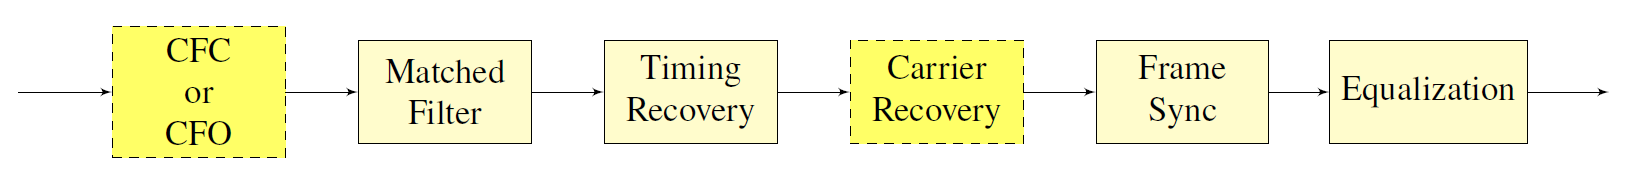
\includegraphics[width=0.8\textwidth]{receiver_block_diagram.png}}}
	\caption{Receiver Block Diagram}
	\label{fig::receiver_block_diagram}
\end{figure}

\subsection{System and Error Models}

In this experiment, we analyze a model of the receiver included in \texttt{lab6part1.m}. In this script, we model the addition of a carrier offset, $f_o$, as follows:

\begin{equation}
	\label{eq::carrier_freq_offset}
	r(k) = s(k)e^{j(2{\pi}f_okT+\theta)}+n(k) = s(k)e^{j(\omega_okT+\theta)}+n(k)
\end{equation}

\noindent The model also generates power spectral density (PSDs) of the signal before and after the carrier offset.

Using the model, we specifically examine the effects of changing the `filterUpsample` variable, which sets the "analog" oversample rate, to 1. Next, with the original value of `filterUpsample`, we increase the frequency offset in unit steps of $0.1F_s$ from $0.1F_s$ to $1.0F_s$ and explain any observed effects. Then, we examine the code in \texttt{lab6part1.m} and state the reasoning behind incrementing the time vector when applying a frequency offset. Finally, we identify sources of the frequency offset besides LO mismatches.

\subsection{Coarse Frequency Correction}

In this experiment, we use a non-data aided (NDA) FFT-based technique for coarse frequency compensation. In this algorithm, we remove the PSK modulation from our received data by raising it to a power equal to modulation order. If we take an FFT of this data, the peak FFT bin should give us the frequency offset multiplied by the modulation order. For BPSK, specifically, we can estimate the frequency offset as follows:

\begin{equation}
	\label{eq::bpsk_coarse_freq_est}	
	\hat{f}_0 = \frac{1}{2TK}\underset{f}{\text{argmax}}\left\vert\sum_{k=0}^{K-1}{r^2(k)e^{-j2{\pi}kT/K}}\right\vert
\end{equation}

\noindent where $K$ is the FFT size and $T$ is the sampling period.

Using Equation \ref{eq::bpsk_coarse_freq_est} as reference, we implement a coarse frequency correction function in MATLAB using the \texttt{fft} function. To test our function, we use signals generated by \texttt{lab6part1.m}. Then, we modify Equation \ref{eq::bpsk_coarse_freq_est} to handle a QPSK signal instead of a DBPSK signal. Finally, we create a function which implements coarse frequency correction for arbitrary PSK modulation orders.

\subsection{Fine Frequency Correction}

In this experiment, we perform fine frequency compensation. The block we implement is designed to compensate for any residual phase or frequency offsets remaining after coarse frequency compensation. The algorithm we implement is specifically illustrated in Figure \ref{fig::fine_freq_comp_block_diagram}.

\begin{figure}[H]
	\centerline{\fbox{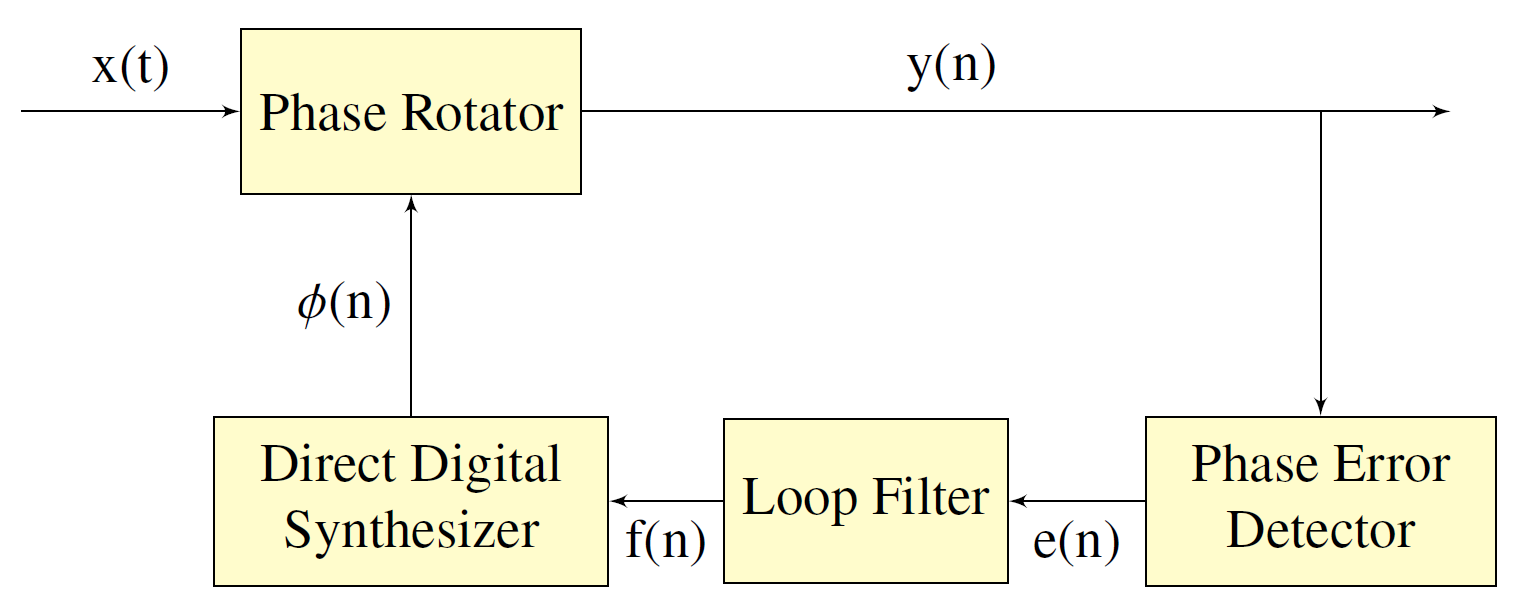
\includegraphics[width=0.6\textwidth]{fine_freq_comp_block_diagram.png}}}
	\caption{Fine Frequency Compensation}
	\label{fig::fine_freq_comp_block_diagram}
\end{figure}

In the block diagram, the phase error detector (PED) measures the phase offset of the received samples. The loop filter governs the dynamics of the PLL. It sets the operational frequency range, lock time, and dampness/responsiveness of the PLL. Finally, the direct digital synthesizer (DDS) generates the correction signal, which is applied by the phase rotator.

The error signal output by the PED is dependent on the modulation scheme. For DBPSK modulation, it is specifically given by:

\begin{equation}
e(k) = \text{sign}(\text{Re}(y(k))) \times \text{Im}(y(k))
\end{equation}

\noindent The loop filter is a proportional-plus-integrator (PI) filter of the following form:

\begin{equation}
F(z) = G_1 + \frac{G_2}{1-z^{-1}}
\end{equation}

\noindent The gain values $G_1$ and $G_2$ are chosen based on a damping factor $\zeta$ and a loop bandwidth $B_\text{Loop}$:

\begin{align}
	\theta = \frac{B_{\text{Loop}}}{M(\zeta + 0.25/\zeta)} && \Delta = 1 + 2\zeta\theta + \theta^2
\end{align}

\begin{align}
	G_1 = \frac{4\zeta\theta/\Delta}{M} && G_2 = \frac{(4/M)\theta^2/\Delta}{M}
\end{align}

\noindent where $M$ is the constellation order. The selection of $\zeta$ affects the responsive and stability of the PLL:

\begin{equation}
\zeta = \begin{cases}
< 1, & \text{Underdamped}\\
= 1, & \text{Critically Damped}\\
> 1, & \text{Overdamped}
\end{cases}
\end{equation}

\noindent $B_\text{Loop}$ is then chosen to achieve a maximum frequency pull-in range, $\Delta_{f,\text{pull}}$, and a maximum frequency lock delay, $t_{\Delta,\text{Max}}$.

%\begin{equation}
%	\Delta_{f,\text{lock}} = \frac{4(2\pi\sqrt{2}\zeta{B_\text{Loop}})^2}{B_\text{Loop}^3}
%\end{equation}

\begin{equation}
	\label{eq::max_freq_correct}
	\Delta_{f,\text{pull}} \sim 2\pi\sqrt{2}\zeta{B_\text{Loop}}\end{equation}

\begin{equation}
	t_{\Delta,\text{Max}} \sim \frac{32\zeta^2}{B_\text{Loop}}\end{equation}
	
Using the provided equations as template, we implement fine frequency compensation (FFC) in MATLAB. We use data from \texttt{lab6part2.m} to validate our design. Next, we evaluate how the convergence times for our function are affected by different damping factors $\zeta$ and loop bandwidths $B_\text{Loop}$. Then, we compare the phase-corrected constellation to the ideal constellation using an error vector magnitude (EVM) metric, which can be computed as follows:

\begin{equation}
	\text{EVM}_\text{RMS} = 100 \times \sqrt{\frac{\frac{1}{N}\sum_{k=0}^{N-1}{e_\text{const}(k)}}{\frac{1}{N}\sum_{k=0}^{N-1}{(\text{Re}(y(k))^2 + \text{Im}(y(k))^2)}}}
\end{equation}

\noindent with

\begin{equation}
	e_\text{const}(k) = (\text{Re}(y(k)) - \text{Re}(\tilde{y}(k))^2 + (\text{Im}(y(k)) - \text{Im}(\tilde{y}(k)))^2
\end{equation}

\noindent and $\tilde{y}(k)$ defined as the reference symbol for $y(k)$. Note that we also can express the EVM in decibels as follows:

\begin{equation}
	\text{EVM}_\text{dB} = 20\text{log}_{10}(\text{EVM}_\text{RMS}/100)
\end{equation}

\noindent Finally, once we complete our EVM measurements, we figure out how the PED would have to change to support QPSK modulation.

\section{Results}
% Results and discussion of the laboratory experiment, including captured outputs, observations, and responses to laboratory questions.

In this section, we highlight the results from each of our experiments. We specifically model carrier frequency offsets. Then, we compensate for the frequency offsets using coarse and fine frequency correction.

\subsection{System and Error Models}

In this experiment, we use Equation \ref{eq::carrier_freq_offset} to model our received signal with a carrier frequency offset. We can use the following DTFT property to examine the spectrum after multiplying the received signal by a complex exponential:

\begin{equation}
	h[n]e^{j\omega_on} = H\left(e^{j(\omega-\omega_o)}\right)
\end{equation}

\noindent Examining the equation, we see that multiplying the signal by a complex exponential results in a shift in the frequency domain. However, because the DTFT is periodic with a period of $2\pi$, it can be more insightful to treat the frequency shift as an circular shift in the frequency-domain. 

As long as the passband of our spectrum does not wrap when apply the frequency offset, our model will generate a spectrum that is representative of a continuous-time frequency shift. Increasing the excess bandwidth allows us to support a larger range of frequency offsets. However, if we change the `filterUpsample' in \texttt{lab6part1.m} to 1, we do have any excess bandwidth. The spectrum after a frequency shift of $0.1F_s$ is shown in Figure \ref{fig::psd_upsample_1}.

\begin{figure}[H]
	\centerline{\fbox{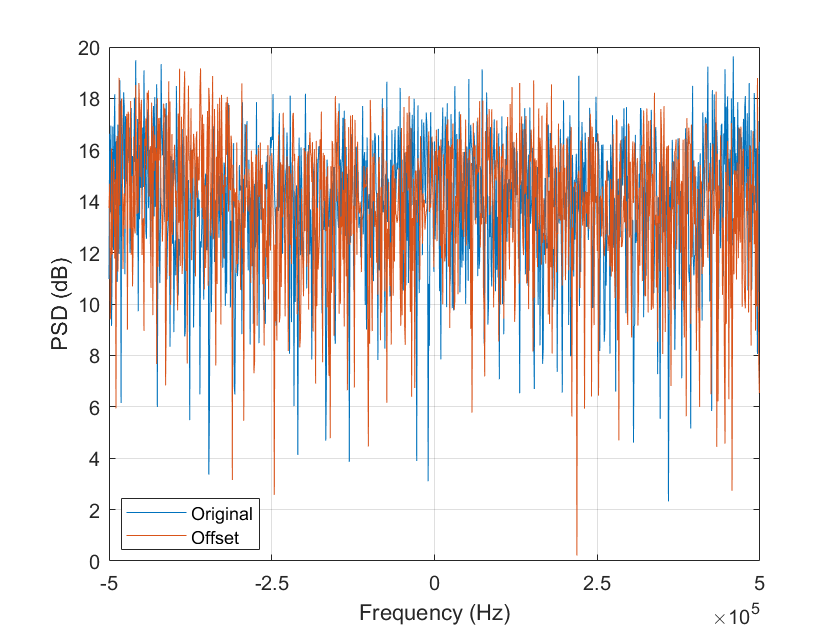
\includegraphics[width=0.5\textwidth]{psd_upsample_1.png}}}
	\caption{Frequency Response with `filterUpsample' Set to 1 and a $\protect{0.1F_s}$ Frequency Shift}
	\label{fig::psd_upsample_1}
\end{figure}

\noindent Examining the frequency response, we see that it does not correctly model a $0.1F_s$ continuous-time frequency shift, which would have resulted in part of the spectrum being zero. Note that our updated frequency response is also not a shift of the original DFT samples. This is because the DFT is sampling the DTFT. With a frequency shift of $0.1F_s$, our updated sampling positions do not align with our initial sampling positions. This results in a a slightly different response. If we instead chose a frequency shift of $F_s/16$, our sampling positions will align, and our DFTs will be related by a circular shift. These results are captured in Figure \ref{fig::psd_upsample_1_mod_shift}.

\begin{figure}[H]
	\centerline{\fbox{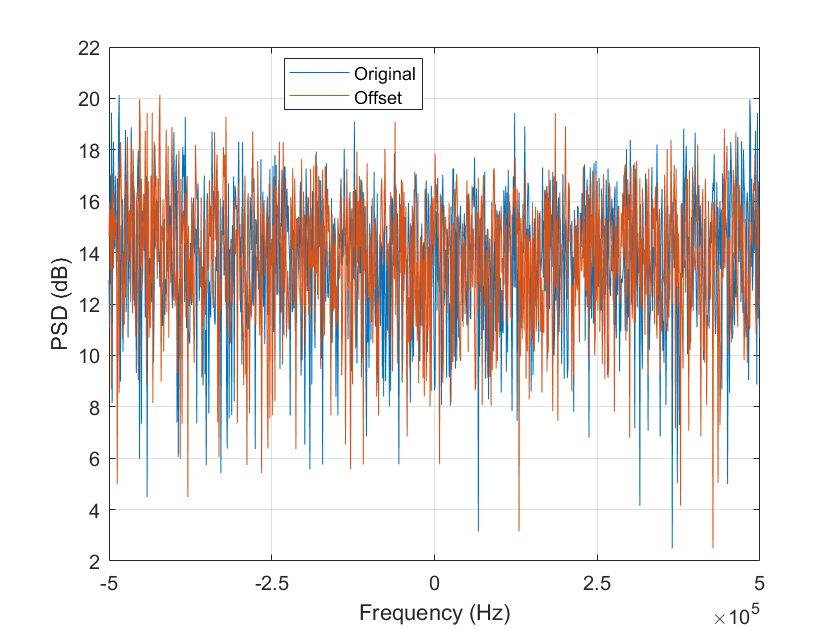
\includegraphics[width=0.5\textwidth]{psd_upsample_1_mod_shift.png}}}
	\caption{Frequency Response with `filterUpsample' Set to 1 and a $\protect{F_s/16}$ Frequency Shift}
	\label{fig::psd_upsample_1_mod_shift}
\end{figure}

\noindent We also observe a similar effect when we step the frequency offset in steps of $0.1F_s$ from $0.1F_s$ to $1.0F_s$. As we increase the frequency offset, we see the frequency response wraps. In Figure \ref{fig::psd_freq_offset_05}, we specifically show the frequency response with a frequency offset of $0.5F_s$. 

\begin{figure}[H]
	\centerline{\fbox{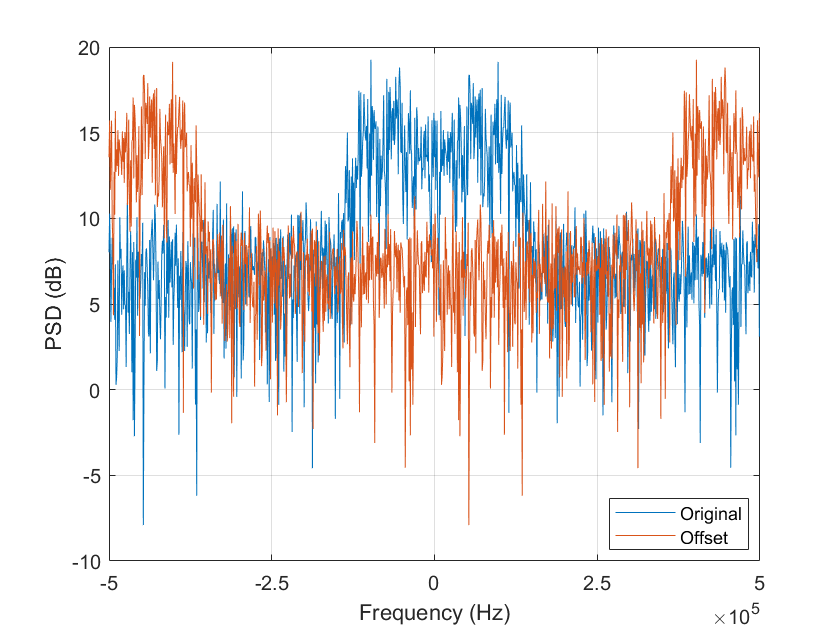
\includegraphics[width=0.5\textwidth]{psd_freq_offset_05.png}}}
	\caption{Frequency Response with a $\protect{0.5F_s}$ Frequency Shift}
	\label{fig::psd_freq_offset_05}
\end{figure}

\noindent At this frequency offset, we see that the frequency response is circularly shifted by half the bandwidth of the signal. We can explain this with DTFT properties as we did previously. However, another equivalent way of explaining these results is to treat the frequency shift as a continuous-time frequency shift followed by sampling. When the highest frequency of the continuous-time signal exceeds half the sample rate, this results in aliasing, which in turn, causes our frequency response to wrap.

	In simulation, we also increment the timing vector for each frame (\texttt{timeIndex = (k:k+frameSize-1).'}). This models back-to-back frames being fed into a free-running oscillator. The frequency offsets we observe are primarily caused by LO mismatches. However, another cause of the frequency offset is a doppler shift (which is caused by relative motion of the receiver with respect to the transmitter).

\subsection{Coarse Frequency Correction}

In this section, we perform coarse frequency correction using an FFT. To remove the modulation from our constellation, we raise our received data up to a power equivalent to the modulation order. The maximum FFT bin then gives us an index that is proportional to our estimated carrier offset. For DBPSK, the estimated carrier offset is specifically given by

\begin{equation}
	\hat{f}_0 = \frac{1}{2TK}\underset{f}{\text{argmax}}\left\vert\sum_{k=0}^{K-1}{r^2(k)e^{-j2{\pi}kT/K}}\right\vert
\end{equation}
	
\noindent When we apply coarse frequency compensation to a DBPSK-modulated signal with a $0.1F_s$ frequency offset, we obtain the spectrum shown in Figure \ref{fig::psd_bpsk_with_cfc}.

\begin{figure}[H]
	\centerline{\fbox{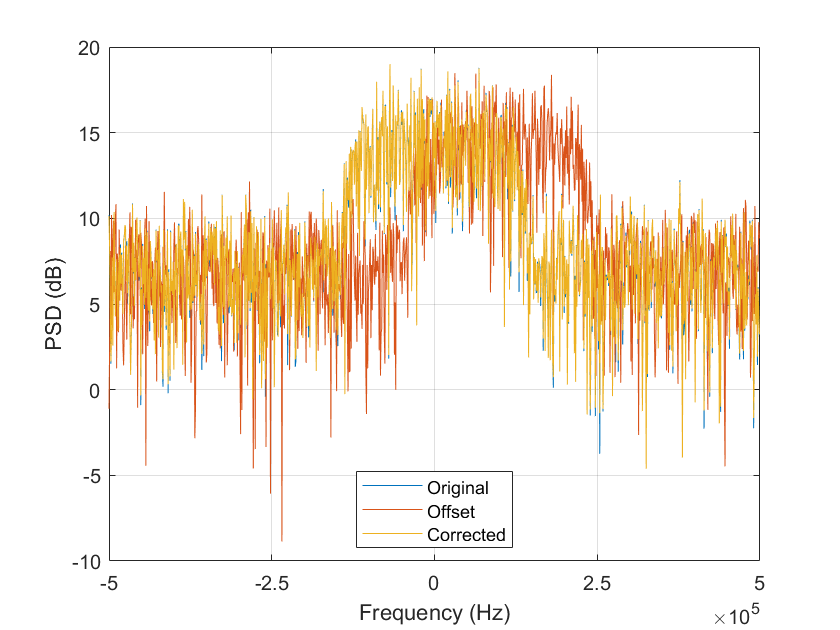
\includegraphics[width=0.5\textwidth]{psd_bpsk_with_cfc.png}}}
	\caption{DBPSK Frequency Response Before and After Coarse Frequency Correction}
	\label{fig::psd_bpsk_with_cfc}
\end{figure}

\noindent Examining the figure, we see that coarse frequency correction effectively removes the carrier offset. Our spectrum before and after compensation is essentially the same. Next, we modify our frequency offset calculation to support QPSK instead of BPSK. The resulting equation is included below:

\begin{equation}
	\hat{f}_0 = \frac{1}{4TK}\underset{f}{\text{argmax}}\left\vert\sum_{k=0}^{K-1}{r^4(k)e^{-j2{\pi}kT/K}}\right\vert
\end{equation}

\noindent Compared to our original equation, we raise our constellation points up to the 4th power instead of the 2nd power to remove the modulation. Next, we we compute our frequency offset, we have to scale the result by 1/4 instead of 1/2 to account for raising our received data to the 4th power instead of the 2nd power. When we apply coarse frequency compensation to a QPSK-modulated signal with a $0.1F_s$ frequency offset, we obtain the spectrum shown in Figure \ref{fig::psd_qpsk_with_cfc}.
 
\begin{figure}[H]
	\centerline{\fbox{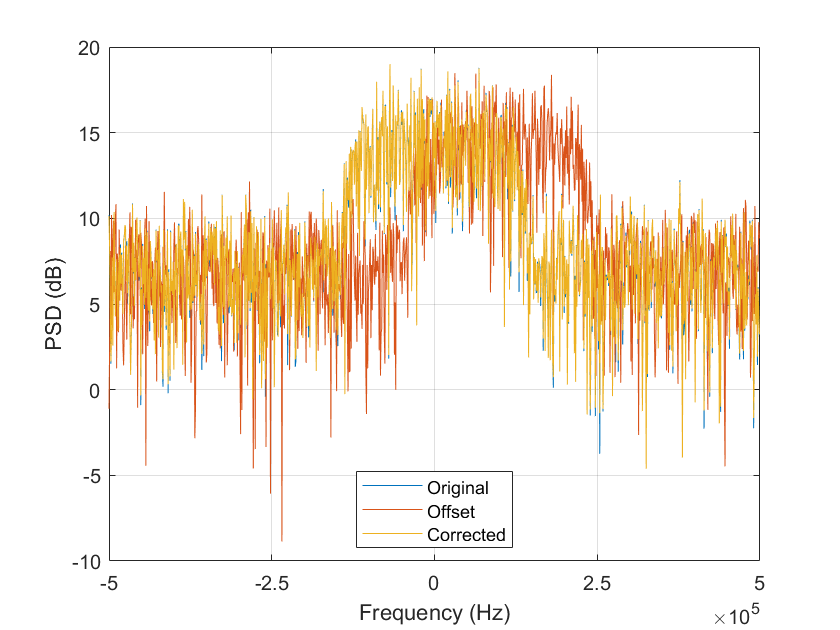
\includegraphics[width=0.5\textwidth]{psd_bpsk_with_cfc.png}}}
	\caption{QPSK Frequency Response Before and After Coarse Frequency Correction}
	\label{fig::psd_qpsk_with_cfc}
\end{figure}

\noindent Examining the resulting figure, we see that our updated equation correctly compensates for a coarse frequency offset in QPSK-modulated data.

\subsection{Fine Frequency Correction}

In this experiment, we perform fine frequency correction on a DPBPSK signal with a 20Hz frequency offset and 15 dB SNR. With $B_\text{loop} = 0.01$ and $\zeta = 1/\sqrt{2}$, our constellation before and after correction is shown in Figure \ref{fig::fine_freq_comp_bpsk_const}.

\begin{figure}[H]
	\centerline{\fbox{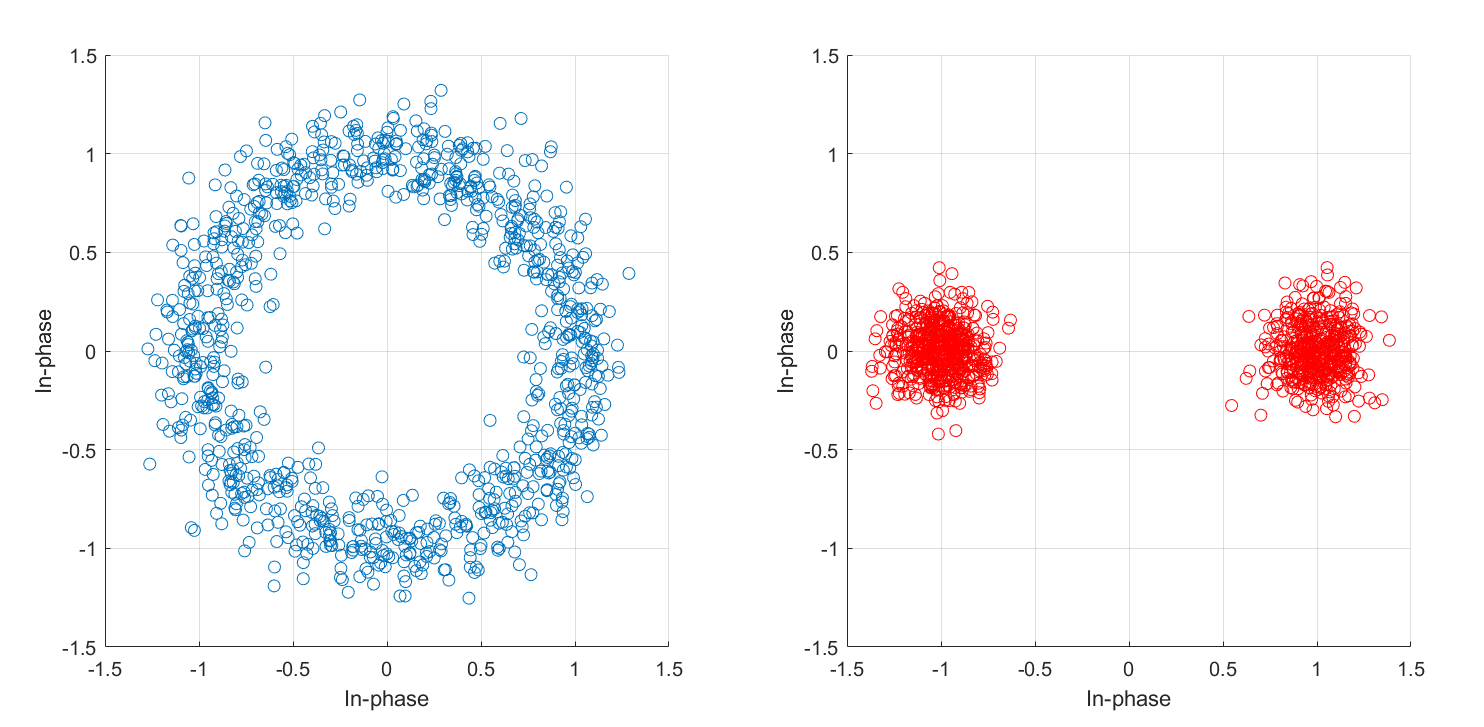
\includegraphics[width=0.8\textwidth]{fine_freq_comp_bpsk_const.png}}}
	\caption{DBPSK Constellation Before and After Fine Frequency Compensation}
	\label{fig::fine_freq_comp_bpsk_const}
\end{figure}

\noindent Qualitatively examining the figure, we see that the frequency offset has been effectively removed. We can quantify the error before and after compensation using the error vector magnitude. However, before we do this, we must handle the phase ambiguity. Our correction algorithm only ensures that our received data lines up with a constellation point (not specific constellation points). For BPSK this means that our compensated data is ambiguous by $180^{\circ}$. For a first-pass implementation, we select the phase ambiguity that minimizes the EVM. This approach over the entire data set is not realizable. However, we can perform it on a smaller scale using code words. Other approaches include differential encoding and equalization. After compensating for the phase ambiguity, we find that our EVM before compensation is 3.09 dB and our EVM after compensation is -14.72 dB.

  The constellation and EVM illustrate the steady state response of the PLL. However, we can plot the frequency output of the PLL to evaluate convergence times. The PLL estimate for the default parameters of $B_\text{loop} = 0.01$ and $\zeta = 1/\sqrt{2}$ is included in Figure \ref{fig::convergence_Bloop_0p01_damp_sqrt_2}.

\begin{figure}[H]
	\centerline{\fbox{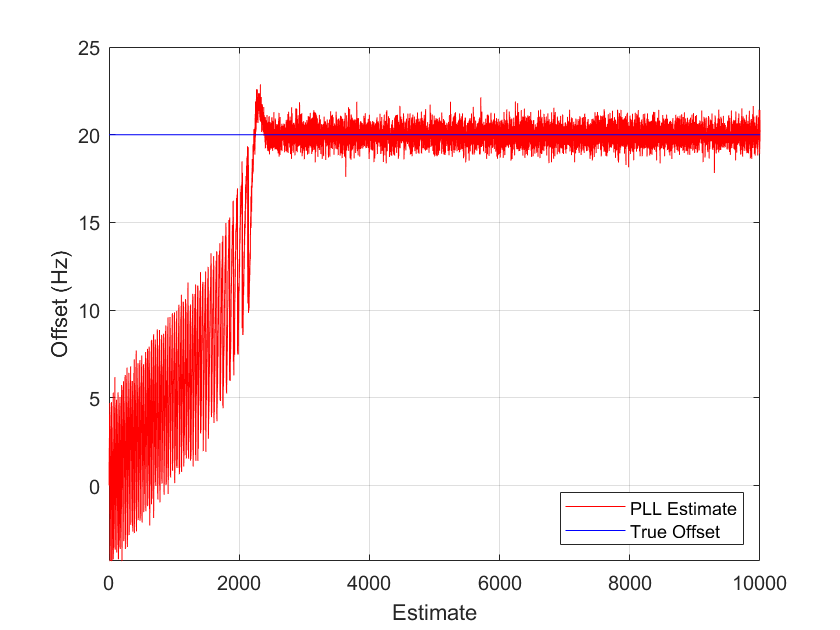
\includegraphics[width=0.5\textwidth]{convergence_Bloop_0p01_damp_sqrt_2.png}}}
	\caption{Plot of PLL Estimate for $\protect{B_\text{loop}} = 0.01$ and $\protect{\zeta = 1/\sqrt{2}}$}
	\label{fig::convergence_Bloop_0p01_damp_sqrt_2}
\end{figure}

\noindent At $\zeta = 1/\sqrt{2}$, the steady-state error variance $\sigma_e=0.307395$. Additionally, the response is underdamped, which leads to ringing. We can exacerbate this ringing by choosing $\zeta=0.25$. The response that results is shown in Figure \ref{fig::convergence_Bloop_0p01_damp_0p25}.

\begin{figure}[H]
	\centerline{\fbox{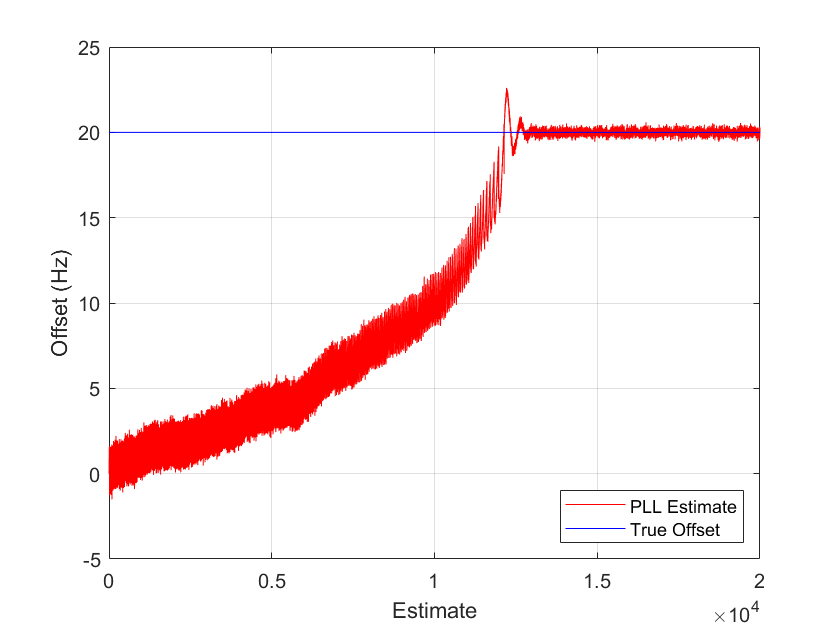
\includegraphics[width=0.5\textwidth]{convergence_Bloop_0p01_damp_0p25.png}}}
	\caption{Plot of PLL Estimate for $\protect{B_\text{loop}} = 0.01$ and $\protect{\zeta = 0.25}$}
	\label{fig::convergence_Bloop_0p01_damp_0p25}
\end{figure}

\noindent Examining the figure, we see that ringing increases as expected. We also find that the convergence time increases by a factor of 5. At steady state, the error variance $\sigma_e=0.0303656$. The decrease in error variance, results in an EVM of -14.74 dB. However, this is nearly identical to our first measurement. This is because our error is dominated by the AWGN instead of the phase error. We also examine the response for $\zeta = 1$, when the system is critically damped. The updated response is included in Figure \ref{fig::convergence_Bloop_0p01_damp_1}.

\begin{figure}[H]
	\centerline{\fbox{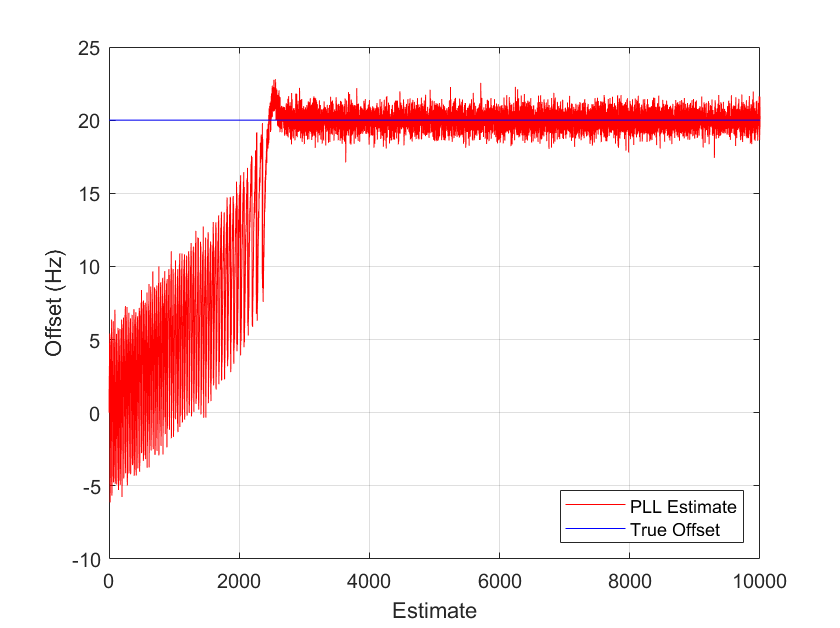
\includegraphics[width=0.5\textwidth]{convergence_Bloop_0p01_damp_1.png}}}
	\caption{Plot of PLL Estimate for $\protect{B_\text{loop}} = 0.01$ and $\protect{\zeta = 1}$}
	\label{fig::convergence_Bloop_0p01_damp_1}
\end{figure}

\noindent Examining the response, we see that the ringing is almost non-existent. The convergence time is also roughly the same as $\zeta = 1/\sqrt{2}$. This is expected result because the system is critically damped at $\zeta = 1$. In other words, the response is as fast as possible without ringing. The error variance $\sigma_e=0.436734$. Similar to our previous results, the EVM after compensation is -14.72 dB because our error is dominated by the AWGN. Next, we examine the response for $\zeta = 2$. Our results are shown in Figure \ref{fig::convergence_Bloop_0p01_damp_2}.

\begin{figure}[H]
	\centerline{\fbox{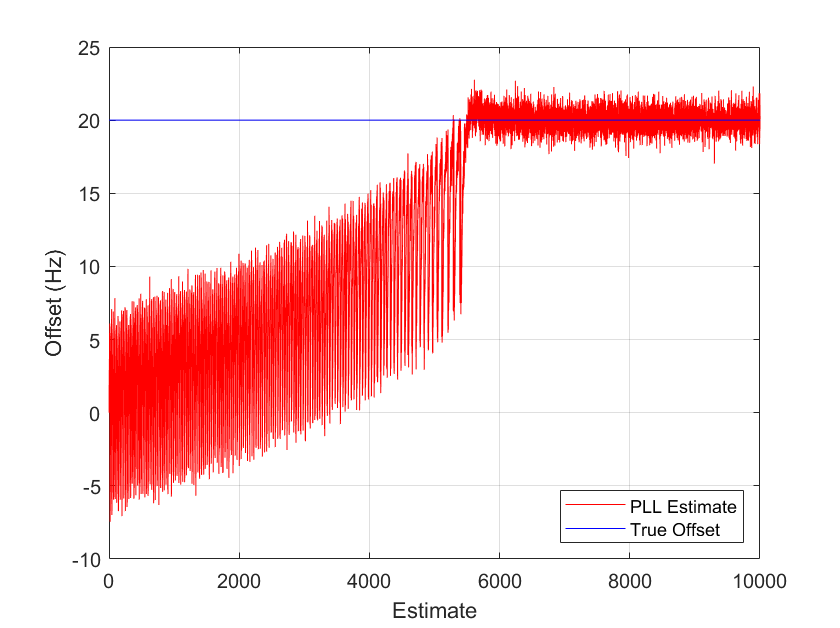
\includegraphics[width=0.5\textwidth]{convergence_Bloop_0p01_damp_2.png}}}
	\caption{Plot of PLL Estimate for $\protect{B_\text{loop}} = 0.01$ and $\protect{\zeta = 2}$}
	\label{fig::convergence_Bloop_0p01_damp_2}
\end{figure}

\noindent Compared to results with $\zeta = 1$, we also do not observe ringing. However, the convergence time increases, which is expected for an underdamped system. The error variance $\sigma_e$ increases to 0.596969. Because the error is dominated by the AWGN, our EVM remains unchanged at -14.72 dB.

Next, we can examine the response when we modify the loop bandwidth, $B_\text{loop}$ instead of the damping factor, $\zeta$. Our results for $B_\text{loop} = 0.005$ and $B_\text{loop} = 0.02$ are included in Figures \ref{fig::convergence_Bloop_0p005_damp_sqrt_2} and \ref{fig::convergence_Bloop_0p02_damp_sqrt_2} respectively.

\begin{figure}[H]
	\centerline{\fbox{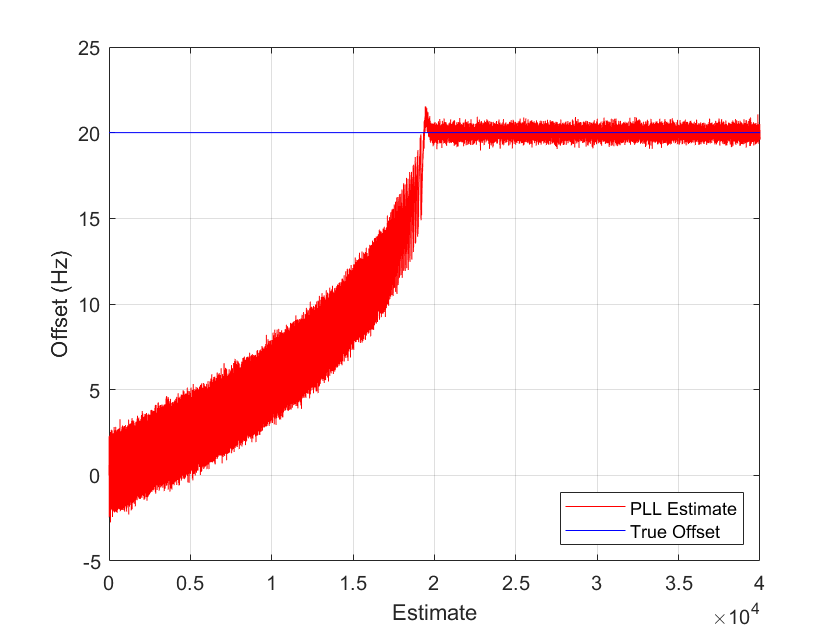
\includegraphics[width=0.5\textwidth]{convergence_Bloop_0p005_damp_sqrt_2.png}}}
	\caption{Plot of PLL Estimate for $\protect{B_\text{loop}} = 0.005$ and $\protect{\zeta = 1/\sqrt{2}}$}
	\label{fig::convergence_Bloop_0p005_damp_sqrt_2}
\end{figure}

\begin{figure}[H]
	\centerline{\fbox{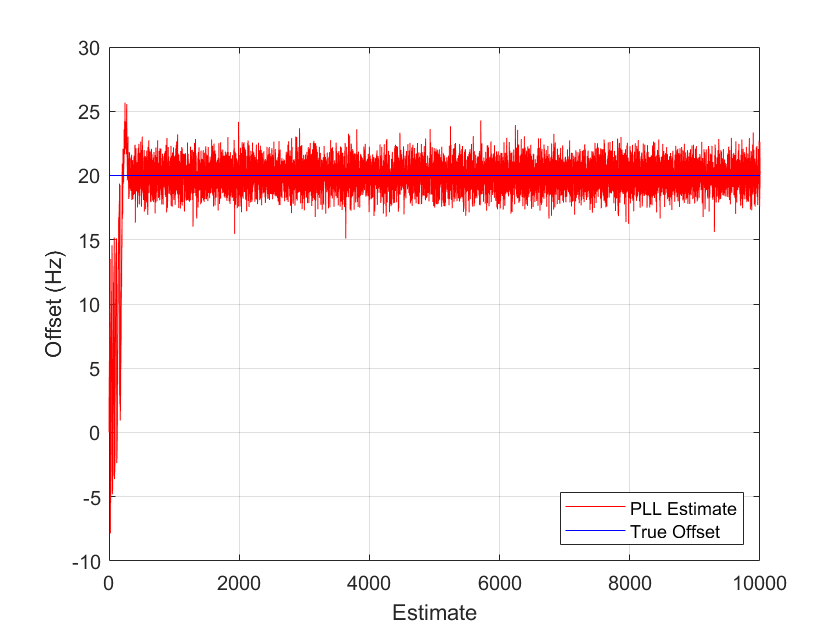
\includegraphics[width=0.5\textwidth]{convergence_Bloop_0p02_damp_sqrt_2.png}}}
	\caption{Plot of PLL Estimate for $\protect{B_\text{loop}} = 0.02$ and $\protect{\zeta = 1/\sqrt{2}}$}
	\label{fig::convergence_Bloop_0p02_damp_sqrt_2}
\end{figure}

\noindent Comparing the responses to our previous response in Figure \ref{fig::convergence_Bloop_0p01_damp_sqrt_2}, we see that a lower loop bandwidth increases the convergence time, while a larger loop bandwidth decreases the convergence time. Additionally, we see that smaller loop bandwidths lead to less error in the response. Compared to our results with $B_{\text{loop}} = 0.01$, we achieve an error variance $\sigma_e=0.134348$ for $B_{\text{loop}} = 0.005$ and an error variance $\sigma_e=2.12314$ for $B_{\text{loop}} = 0.02$. In other words, our frequency estimate improves as we decrease the loop bandwidth. However, this error variance has minimal effects on our EVM because of the high noise floor. With $B_{\text{loop}} = 0.005$, we measure an EVM of -14.74 dB, and with $B_{\text{loop}} = 0.02$, we measure an EVM of -14.67 dB. 

Interestingly, when we increase SNR, the EVM relationships remain approximately the same. At a 60 dB SNR for example, we measure an EVM of -59.74 dB with $B_{\text{loop}} = 0.005$, -59.72 dB with $B_{\text{loop}} = 0.01$, and -59.67 dB with $B_{\text{loop}} = 0.02$. Thus, our EVM is nearly independent of $B_{\text{loop}}$ for static frequency offsets. Our EVM results, however do to start to differ if we add a frequency drift. This is due to different convergence times for each selection $B_{\text{loop}}$. If we consider a 1Hz/s drift at 15 dB SNR, our response with $B_{\text{loop}} = 0.01$ and $\zeta = 1/\sqrt{2}$ is given below.

\begin{figure}[H]
	\centerline{\fbox{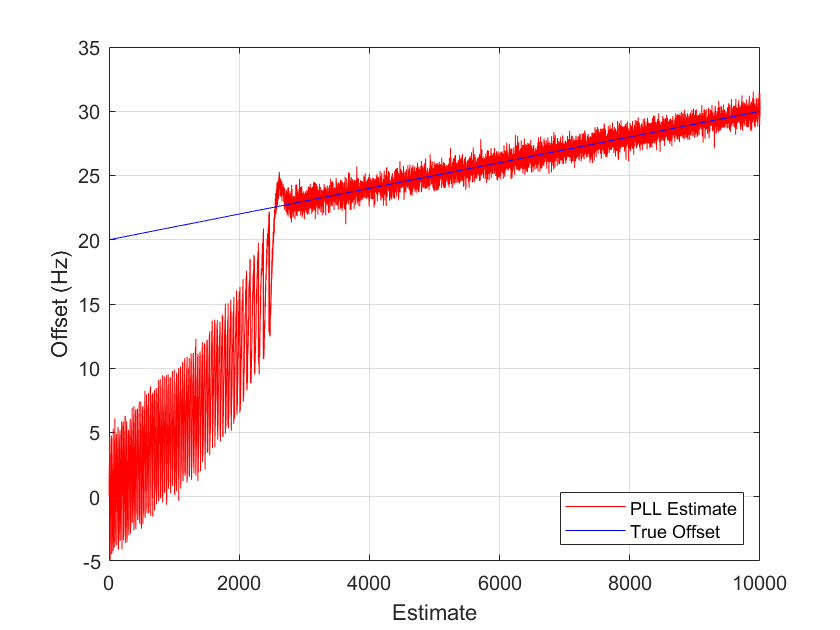
\includegraphics[width=0.5\textwidth]{convergence_1Hz_drift_Bloop_0p01_damp_sqrt_2.png}}}
	\caption{Plot of PLL Estimate with 1 Hz/s drift, $\protect{B_\text{loop}} = 0.01$, and $\protect{\zeta = 1/\sqrt{2}}$}
	\label{fig::convergence_1Hz_drift_Bloop_0p01_damp_sqrt_2}
\end{figure}

\noindent Similarly, we show the results with $B_{\text{loop}} = 0.005$ and $\zeta = 1/\sqrt{2}$ below:

\begin{figure}[H]
	\centerline{\fbox{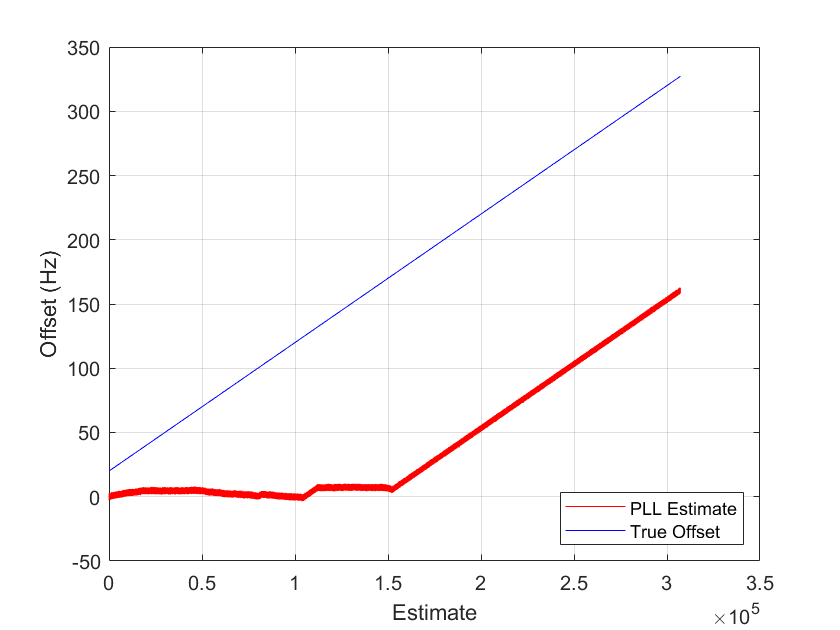
\includegraphics[width=0.5\textwidth]{convergence_1Hz_drift_Bloop_0p005_damp_sqrt_2.png}}}
	\caption{Plot of PLL Estimate with 1 Hz/s drift, $\protect{B_\text{loop}} = 0.005$, and $\protect{\zeta = 1/\sqrt{2}}$}
	\label{fig::convergence_1Hz_drift_Bloop_0p005_damp_sqrt_2}
\end{figure}

\noindent Comparing the two figures, we see that the PLL has difficulty keeping up with the frequency drift when $B_\text{loop} = 0.005$. If we measures the EVM, we see that it is -14.68 dB for $B_\text{loop} = 0.01$ and 3.08 dB for $B_\text{loop} = 0.005$. We also increase the SNR to 60 dB to characterize the EVM for $B_\text{loop} = 0.01$ and $B_\text{loop} = 0.02$. Doing so, we measure an EVM of -34.93 dB for $B_\text{loop} = 0.01$ and -46.64 dB for $B_\text{loop} = 0.02$. Thus, our choice of control system parameters becomes more important as our input becomes more dynamic. We specifically note that with a faster-responding control system, we can better handle dynamic inputs with only marginal  performance hits for static frequency offsets.

We also examine how the loop filter parameters influence the maximum correctable frequency. For a 50 Hz offset with $B_{\text{loop}} = 0.01$ and $\zeta = 1/\sqrt{2}$, the PLL response is shown in Figure \ref{fig::convergence_Bloop_0p01_damp_sqrt_2_foff_50}.

\begin{figure}[H]
	\centerline{\fbox{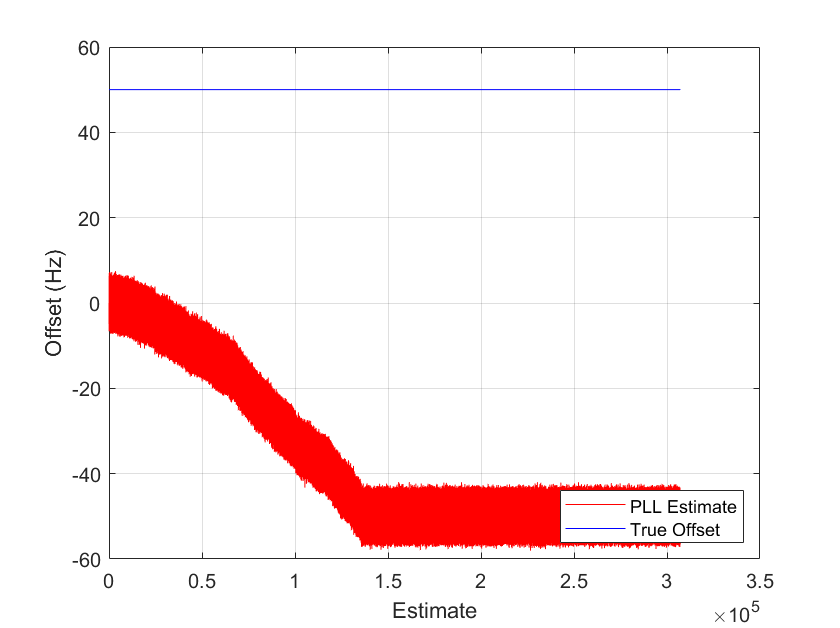
\includegraphics[width=0.5\textwidth]{convergence_Bloop_0p01_damp_sqrt_2_foff_50.png}}}
	\caption{Plot of PLL Estimate with 50 Hz Frequency Offset, $\protect{B_\text{loop}} = 0.01$, and $\protect{\zeta = 1/\sqrt{2}}$}
	\label{fig::convergence_Bloop_0p01_damp_sqrt_2_foff_50}
\end{figure}

\noindent Examining the response, we see that the PLL fails to lock. If we increase $B_{\text{loop}}$ to 0.05 and $\zeta$ to 2, we get the results shown in Figure \ref{fig::convergence_Bloop_0p05_damp_2_foff_50}.

\begin{figure}[H]
	\centerline{\fbox{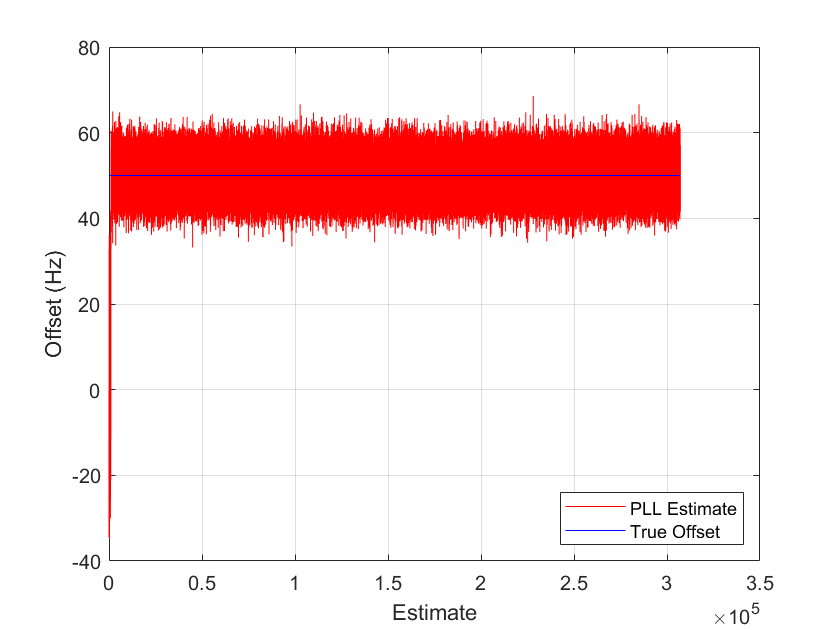
\includegraphics[width=0.5\textwidth]{convergence_Bloop_0p05_damp_2_foff_50.png}}}
	\caption{Plot of PLL Estimate with 50 Hz Frequency Offset, $\protect{B_\text{loop}} = 0.05$, and $\protect{\zeta = 2}$}
	\label{fig::convergence_Bloop_0p05_damp_2_foff_50}
\end{figure}

\noindent Comparing the results to Figure \ref{fig::convergence_Bloop_0p01_damp_sqrt_2_foff_50}, we see that the PLL now converges. This is consistent with Equation \ref{eq::max_freq_correct}, which states that the maximum correctable frequency increases with increasing  $B_{\text{loop}}$ and $\zeta$. Note that our results did not seem to indicate a linear relationship between the maximum resolve frequency and $B_{\text{loop}}$ or $\zeta$. This is likely because Equation \ref{eq::max_freq_correct} makes some assumptions about the size of the frequency offset with respect to the signal bandwidth that do not hold in this case.

We can modify our PED to support different modulation schemes. For example, to support QPSK modulation, we need to modify the PED to perform the following computation:

\begin{equation}
	e(k) = \text{sign}(\text{Re}(y(k))) \times \text{Im}(y(k)) - \text{sign}(\text{Im}(y(k))) \times \text{Re}(y(k))
\end{equation}

\noindent This modified equation tries to force $\text{Re}(y(k)) = \pm \text{Im}(y(k))$, which forces the data to a QPSK constellation point. Our constellation with a 20 Hz frequency offset and a 15 dB SNR is shown before and after fine frequency correction in Figure \ref{fig::fine_freq_comp_qpsk_const}. For our correction, we reuse our loop filter parameters $B_{\text{loop}}=0.01$ and $\zeta=1/\sqrt{2}$.

\begin{figure}[H]
	\centerline{\fbox{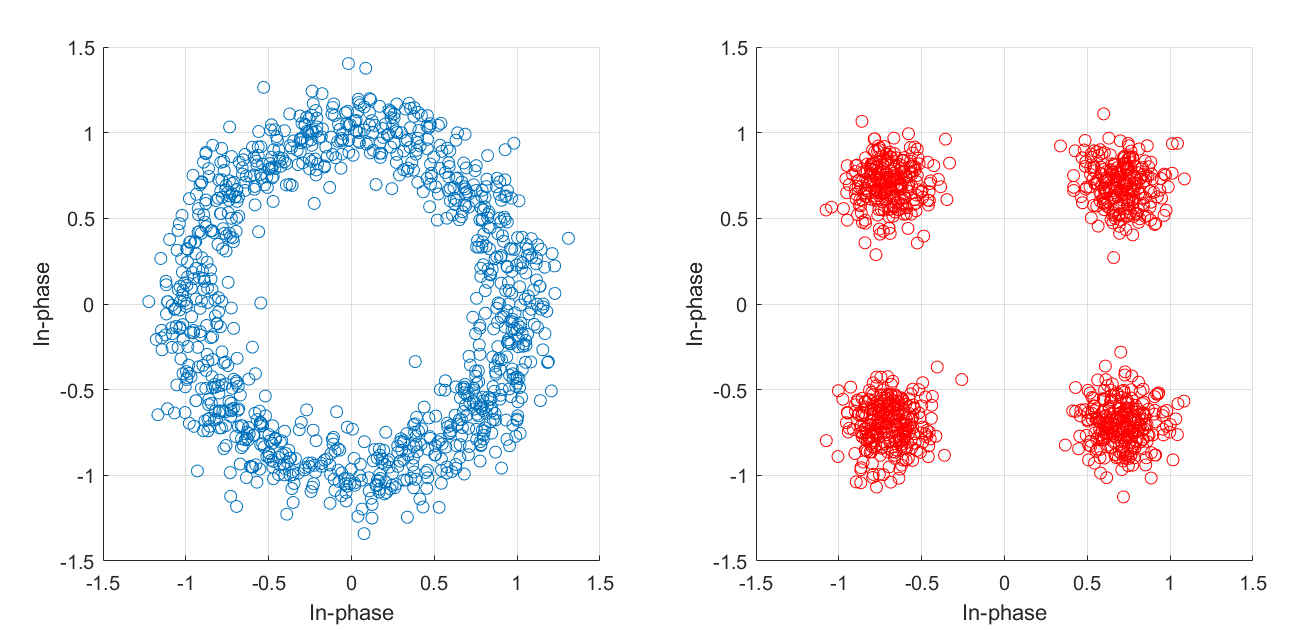
\includegraphics[width=0.8\textwidth]{fine_freq_comp_qpsk_const.png}}}
	\caption{QPSK Constellation Before and After Fine Frequency Compensation}
	\label{fig::fine_freq_comp_qpsk_const}
\end{figure}

\noindent After compensation, we see that our constellation points match our expected QPSK constellation. Additionally, we measure an EVM of 3.07 dB before compensation and -14.75 dB after compensation. Additionally, we show the PLL estimate after compensation, which converges to the correct frequency offset as expected.

\begin{figure}[H]
	\centerline{\fbox{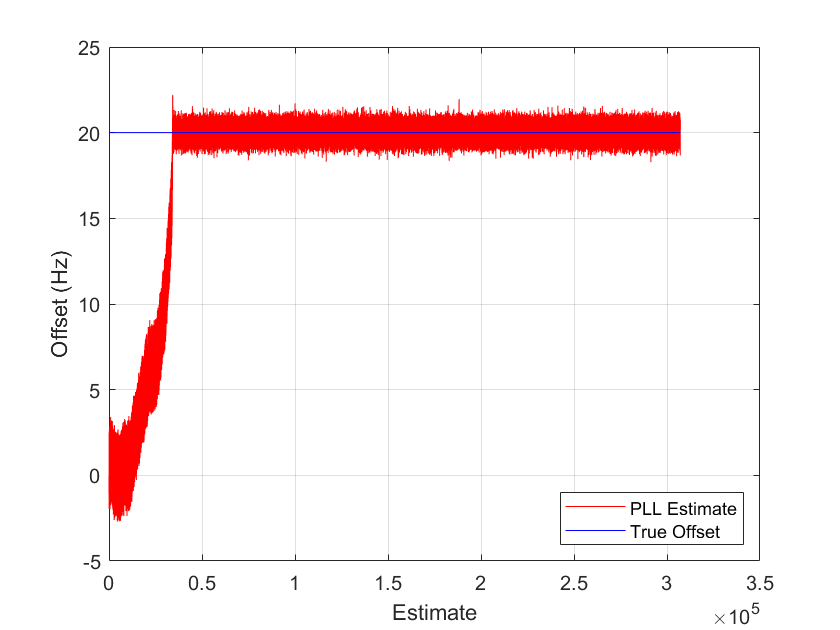
\includegraphics[width=0.5\textwidth]{convergence_qpsk_Bloop_0p01_damp_sqrt_2.png}}}
	\caption{Plot of PLL Estimate for QPSK Modulation with $\protect{B_\text{loop}} = 0.01$ and $\protect{\zeta = 1/\sqrt{2}}$}
	\label{fig::convergence_qpsk_Bloop_0p01_damp_sqrt_2}
\end{figure}

\section{Conclusion}
% Conclusions to the overall lab that discuss meaningful lessons learned and other takeaways from the assignment. (Important)

In this lab, we learned how to model frequency offsets and compensate for them using coarse and fine frequency correction. We modeled frequency offsets in our data by applying a frequency offset in discrete time. Applying the frequency offset in discrete time circularly shifted our spectrum, which differed from an analog frequency shift when significant portions of our spectrum wrapped. This was especially a problem when our upsample rate was 1. Alternatively, we learned that we could treat the discrete frequency shift as an analog frequency shift without a low-pass filter prior to sampling. This resulted in aliasing (frequency wrapping) for large frequency shifts. In this part of the lab, we also learned that the frequency offsets were typically caused by LO mismatches but could also occur due to environmental factors such as doppler shifts.

To compensate for this frequency offset, we used a two-stage design. The first stage course, coarse frequency correction, corrected for large frequency offsets, while the second stage, fine frequency correction, corrected for small frequency offsets. The coarse frequency correction logic worked by raising the PSK-modulated data to the modulation order. This removed the modulation and enabled us to perform an FFT to identify the frequency offset.

Then, after removing this offset, we performed fine frequency correction. Our fine frequency correction used a PLL to compensate for the frequency offset. The PLL included a phase error detector (PED), which used a constellation-dependent formula to detect the phase error. This phase error was then fed into a loop filter, which used a PI filter to estimate the phase of the input. This phase estimate was finally fed into the DDS, which integrated the phase and removed it from the input signal. Finally, the phase was input to a phase rotator which multiplied the input by a complex exponential to remove the phase offset.

We specifically investigated how the damping factor and loop bandwidth affected the convergence times. We specifically found the response converged fastest for damping factors just below the critical damping point ($\zeta = 1$). Additionally, we observed overshoot and oscillation in our responses when the system was underdamped ($\zeta < 1$). We also found that the response converged quickest for large loop filter gains $\beta$. However, the frequency error was also largest for large values of $\beta$. However, the EVM increased much slower than the frequency error. We found that we could choose slightly larger values of $\beta$ without significantly degraded performance. The large values of $\beta$ also significantly improved performance for time-varying frequency offsets. Then, we observed how the loop filter bandwidth $\beta$ and damping factor $\zeta$ impacted the maximum frequency locking range. We found that the maximum locking range increased with $\beta$ and $\zeta$ but did not strictly follow the linear relationship given in Equation \ref{eq::max_freq_correct}. Finally, we extended our fine frequency correction to QPSK and showed that it could also effectively remove frequency offsets.

\end{document}